\section{Sensor Heading System}
% A5.1 Construct the complete heading system model in SIMULINK and include the diagram in your report. Also give details of the parameters used in the blocks representing the various subsystems. (10 marks)

The design of a heading directional sensor system is inherently related to the aircraft in which it is installed. Mechanical loads, vibrations, and operational frequencies interfere with electro-mechanical sensors and the outputted electronic signals accordingly. Small or medium sized UAVs also require a an independent heading system when telecommunication is not possible. The fundamental configuration of the integration of a gyroscope and a magnetic compass will be analysed for this scenario and optimal system design metrics are proposed. 

In order to design a low cost system, off-the-shelf components are selected. The magnetic compass is lightly damped due to fluid viscosity, and has a rise time $t_{rise} = 0.4s$ and settling time $t_{settling} = 18s$. Levi et al. \cite{levi2005gyro} describe how traditional magnetic compasses are subject to errors from both local magnetic fields and accelerations due to motion. These can also contribute to further dynamic controls.

% S4.1 Construct a model of a magnetic compass. Represent the compass as a second order system with unity sensitivity, rise time 0.4s and settling time 18s. The input to your compass model will be true heading and the output will be the heading indicated by the compass needle.

% ➢ S4.2 Produce a Bode plot (gain and phase frequency response) of the compass and use this to identify the useable frequency range of this sensor.
Given the step response parameters above, the compass system can be idealized as a second order system in the form of Equation \ref{eq:second_order_differential} in the time domain and Equation \ref{eq:second_order_transfer_function} in the Laplace domain as further where $w_n$ is natural frequency, $\zeta$ is the damping ratio, and $\lambda$ is the response amplitude gain described by \cite{ogata2010modern}. The under-damped equation condition of a damping ratio $\zeta << 1$ is tested and determined to be valid in Equation \ref{eq:second_order_damping_ratio_approximation}. The derived transfer function in Equation \ref{eq:second_order_transfer_function} can be analysed in MATLAB in the frequency domain using bode plots. It provides an indication of the response for several frequencies excitation as observed in Figure \ref{fig:compass_bode_plots}.

\begin{equation}
    \zeta \approx \frac{3}{w_n t_{settling}} 
\approx \frac{3 t_{rise}}{1.02 t_{settling}}
\approx 2.94 \frac{t_{rise}}{t_{settling}} = 0.0666
\label{eq:second_order_damping_ratio_approximation}
\end{equation}

%The 3dB cutoff maximum frequency is limited at a maximum slope of 0.12. The minimum and maximum safe operational frequency of the sensor is:  1.4969 rad/s with a maximum magnitude of 1 dB

\begin{equation}
\ddot{y}(t) +2 \zeta \dot{y} w_n (t) + w_n^2 y(t) = \lambda w_n^2 u(t)
\label{eq:second_order_differential}
\end{equation}

\begin{equation}
\frac{Y(s)}{U(s)} =
\frac{\lambda w^{2}_{n}}{s^2 + 2 \zeta w_n s + w^{2}_{n}} =
\frac{6.25}{s^2 + 0.333s + 6.25} 
\label{eq:second_order_transfer_function}
\end{equation}

Mathematically it is known from the bode plots that the compass system operates linearly at low mechanical frequencies. To analytically derive this linear range of the response below 3dB, the slopes between the plot sample points were taken to determine their limit closer to 0. All the green points within the magnitude analytic bode plot have a slope between the points of 0.15, and the maximum linear response at this position occurs at 1.29 $rad$ with a magnitude of 2.59 $dB$. If the linear slope restriction would be lowered to 0.12, for example, the maximum response in this line would be at the sampled point of 1.04 $rad$ with a maximum magnitude of 1.4969 $dB$. The frequency response of the compass becomes nonlinear since it has a resonance at the natural frequency $w_n$. The resonant point is achieved at 2.55 rad with a magnitude of 16.7 dB. The poles are derived as $p_{1,2} = \zeta w_n \pm jw_n\sqrt{1 - \zeta^2}$ for an under-damped system \cite{ogata2010modern} with the damping ratio approximation described in Equation \ref{eq:second_order_damping_ratio_approximation}. The two horizontal lines in Figure \ref{fig:compass_bode_plots} indicate the -3 $dB$ and + 3 $dB$ range of the response for amplification comparison reference. For the purposes of this sensor model, a transfer function block with these parameters is used in Simulink.

\begin{figure}
    \centering
    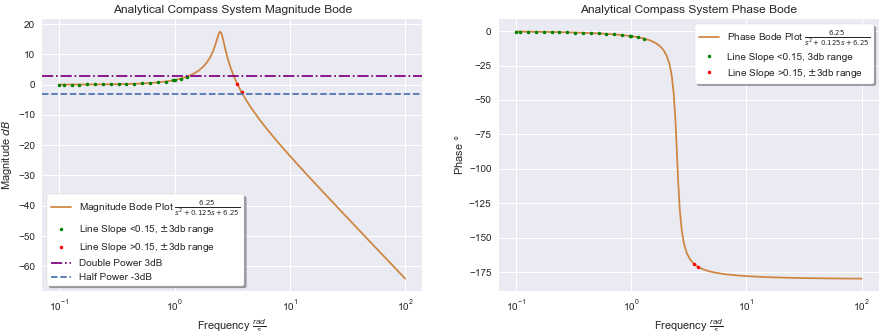
\includegraphics[width=\textwidth]{img/compass_bode_plots.png}
    \caption{Compass Bode Plot}
    \label{fig:compass_bode_plots}
\end{figure}

%S4.3 Construct a model of a gyro compass. Represent the gyro-compass as an ideal sensor with error modelled as integrated white noise with an offset, e.g. Fig. 8.
In order to accurately model the gyro, its mechanical operation needs to be considered. The physical design of a rate gyro is described in Morris \& Langari \cite{MORRIS2016599}, and consists of mainly consists of a spinning wheel attached to a gimbal rotational support that rotates around a fixed static frame of the sensor. The idealised physical behaviour of how this gyro is described in the time domain and Laplace domain is shown in Equation \ref{eq:gyro_transfer_function}. If the spinning mass is has large enough angular momentum $h$, it would mean that large, torques $T$ exerted on the sensor would force small rotation $\Theta_m$ that could be measured by a transducer. Assuming a burst of wind generates torques within the gyro frequency range, destabilizing friction, material stiffness and a limited measurement range could provide inaccurate signals. Hence, low turning rates might not be accurately measured, whereas higher turning rates would.

\begin{equation}
T(s) = {\mathcal {L}}\{h\dot{\theta_m}\} = sh\theta_m
\label{eq:gyro_transfer_function}
\end{equation}

\begin{equation}
\frac{\theta_m}{T} = \frac{1}{sh}
\end{equation}

To model these imperfections within Simulink, a random number with mean of 0.02 and standard deviation of 0.1 would be the equivalent of $\frac{1}{h}$ as observed in Figure \ref{fig:gyro_simulink_block}. A value for $h$ cannot be explicitly determined since this modelling includes random error considerations. This multiplies an integrator block $\frac{1}{s}$. Purely analytically, it is known that the bode plot of an integrator is a line with a negative slope as observed in Figure \ref{fig:gyro_bode}, and it would also have jitter when considering the random mean gain. A discrete Fast Fourier transform could also have performed on the integrator output to obtain this diagram. However, for the purposes of idealistic design, it can already be observed that for a range of frequencies of $10^{-2}$ to $10^{2}$ $rad/s$ the gyro system provides a linear magnitude response with attenuation at faster frequencies. After the $10^{2}$ $rad/s$ point, the gyro would not respond to higher frequencies.


\begin{figure}[H]
\begin{subfigure}{.4\linewidth}
  \centering
  % include first image
  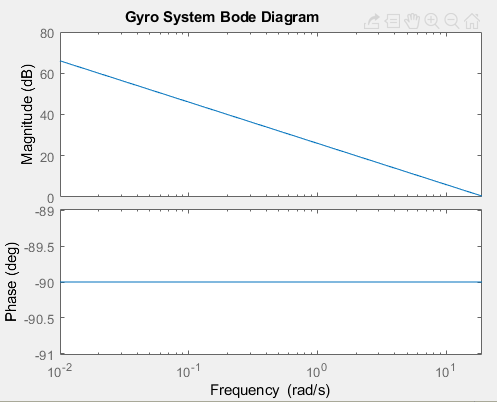
\includegraphics[width=\linewidth]{img/gyro_system_bode.PNG}  
  \caption{Gyro System Bode Plot}
  \label{fig:gyro_bode}
\end{subfigure}
\begin{subfigure}{.6\linewidth}
  \centering
  % include second image
  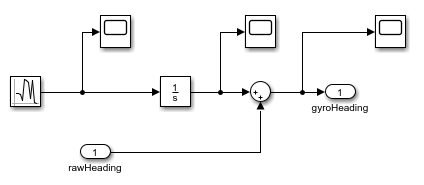
\includegraphics[width=\linewidth]{img/gyro_simulink_block.PNG}  
  \caption{Gyro Simulink block.}
  \label{fig:gyro_simulink_block}
\end{subfigure}
\caption{Gyro Simulink Bode}
\label{fig:fig}
\end{figure}


%➢ S4.4 Sketch the frequency spectrum of the output of the random number block, and the gain frequency response of an integrator, hence sketch the frequency spectrum of the error signal added to the true heading.

% ➢ S4.5 Suggest the useable frequency range of the gyro compass – note it is not possible to quantify in the same way as the magnetic compass

% S4.6 Determine the transfer functions for a pair of complementary first order filters with gain of ‘1’ in the pass band. Choose a suitable cut-off frequency for your filters based on the results of T4.2/T4.5. 
Fox et al. \cite{foxlin1996inertial} demonstrate how sensor fusion through complementary filters integrates responses to minimize individual sensor errors through Kalman algorithms. A simpler, non-probabilistic approach, will be tested by creating complementary filters with the mathematical relationship in Equation \ref{eq:complementary_filters} where the time constant $\tau = \frac{1}{w_{c}}$ is inverse to the cutoff frequency $w_{c}$ in $rad/s$. Since filters have the same cutoff frequency, when the low pass $L(s)$ compass filter response begins diminishing, the high pass $H(s)$ gyro filter magnitude increases. There is no amplification gain from this sensor configuration since its absolute value is unity ($K=1$). The optimal cutoff frequency would reduce the levels of oscillations of the full system signal by making each sensor respond within its ideal operational range. 

\begin{equation}
    L(s) + H(s) =
    \frac{s}{s + \frac{1}{\tau}} +  K{\frac  {1}{\tau s+1}} = 1
    \label{eq:complementary_filters}
\end{equation}



Using all the numerical parameters described previously, sensor fusion was performed and analysed on a magnetic compass and gyroscope as observed in Figure \ref{fig:simulink_model} using Simulink. The selected solver configuration was the variable step ODE-45 with 0.1 sample time was selected since it consistently provided expected results. Although larger sampling times also provided accurate results, computational efficiency was not completely needed for the algorithms in this model. The standard simulation time selected was 350 seconds.

\begin{figure}[h]
    \centering
    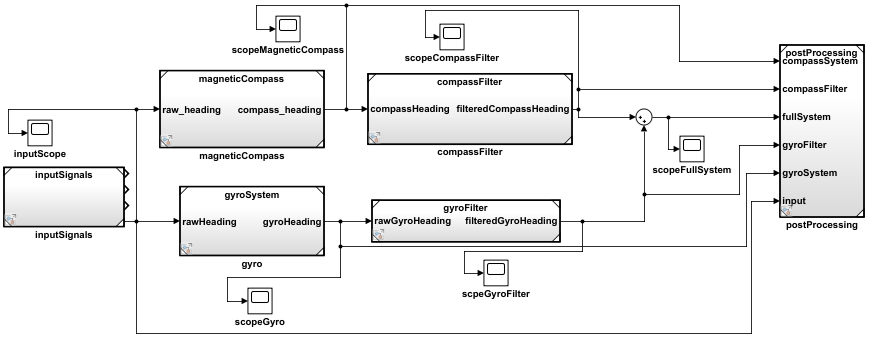
\includegraphics[width=\textwidth]{img/simulink_model.PNG}
    \caption{Heading system Simulink model}
    \label{fig:simulink_model}
\end{figure}

Several improvements could be done to this sensor fusion design to improve its accuracy, and possible future work could be performed analysing its behaviour. Within traditional aircraft navigation, once the rotational motion is negligible, the zero offset of the gyroscope is generally re-tuned, adding some degree of error. Micro-electrically modulated gyroscopes also reduce the zero-offset error, and Kalman auto-correction algorithms could be implemented as described by Levi et al. \cite{levi2005gyro} and Carque et al. \cite{carque2011sensor}. Integrating accelerometers into the heading system can further improve the accuracy of the signal since inertial changes can be considered alongside mobility changes of the gyro at higher frequencies; as described by Young Quist \cite{youngquist1997rate} and Foxlin \cite{foxlin1996inertial}. Lastly, adding extra gyro sensors could potentially add redundancy for the random error in case no other complementary sensors can be added.

% TODO add figure maybe









